\chapter{Tactiques de CAS RWs}

\e
    \item Ce chapitre aborde certaines des tactiques particulières au \gls{rw}. Ces tactiques évoluent en permanence et doivent être adaptées en fonction de la situation.
    \item \important{La décision finale d’utiliser telle ou telle tactique revient toujours au chef de patrouille, mais ce dernier doit veiller à se plier aux contraintes imposées par le \gls{jtac}/\gls{faca}.}
\ed

\section{Altitude d’opération}

\e
    \item Pour une patrouille \acrshort{rw}, on définit l’altitude comme suit:
    %\ee
    	\remark{%
    	\ee
        \item Haut: au dessus de 1000m sol
        \item Moyen: entre 200m et 1000m sol
        \item Bas: en dessous de 200m sol
        \ed
        }%
    %\ed
\ed

\section{Lancement et récupération}

\e
    \item
    Les unités \gls{rw} peuvent opérer à partir de base aérienne ou de points avancés (uniquement les \glspl{farp} dans DCS), ce qui les place au plus près de la ligne de front et prêts à intervenir rapidement.
\ed

\section{Communication durant le transit}

\e
    \item
    Du fait de leur capacité à évoluer à faible altitude, il est souvent difficile pour le \gls{cc} de maintenir une communication constante avec les unités \gls{rw}.
    \item
    Cette difficulté est à prendre en compte lors de la préparation de la mission,  et un système alternatif doit être mis en place pour assurer les communications entre les unités \gls{rw} et leur \gls{tacon}.
\ed

\section{Tactiques durant le transit}

\subsection{Objectifs}

\e
    \item Handicapées par leur faible vitesse, les unités \gls{rw} doivent mettre à profit leur manœuvrabilité pour:
    \ee
        \item Éviter les concentrations de défenses anti-aériennes ennemies
        \item Empêcher la détection le plus longtemps possible
        \item Rester en dehors de la portée de certains systèmes d’armes sol-air
    \ed
\ed

\subsection{Navigation}

\e
    \item Le profil de pénétration (route, altitude, vitesse, formation, suivi du terrain) doit être prévu de manière à atteindre ces objectifs.
    \item En plus des considération purement tactiques, d’autres facteurs entrent en ligne de compte:
    \ee
        \item La météo
        \item Le carburant
        \item Les défenses anti-aériennes alliées
    \ed
    \item Les profils de pénétration possibles sont regroupés en trois catégories:
    \remark{%
    \ee%
        \item Bas niveau: L’approche bas niveau se fait à vitesse et altitude constante (30-60m du sol).%
        \item Contour: Le vol de contour se fait en utilisant le terrain, les obstacles et la végétation pour occulter la formation à l’ennemi, généralement entre 15 et 30 mètres du sol.%
        \item \gls{noe}: Le vol \gls{noe} se fait aussi proche que possible du sol, à des vitesses et altitudes variables, qui dépendent du terrain, de la météo, de la luminosité et de l’ennemi
    \ed%
    }%
\ed

\subsubsection{Menaces particulières}

\e
    \item De par leur très faible altitude de navigation, les \gls{rw} sont vulnérables au tir d’armes de petit calibre et aux \glspl{rpg}.
    \item Certains situations nécessiteront que la patrouille évolue à altitude plus élevée.
    \item Pour ces mêmes raisons, une patrouille \gls{rw} évitera de survoler un environnement urbain (hors phase d’attaque).
\ed

\subsubsection{Jour et nuit}

\e
    \item L’altitude et la vitesse devront être adaptées en fonction de la luminosité ambiante en corrélation avec le type de terrain survolé.
\ed

\section{Tactiques de pénétration}

\e
    \item Les tactiques de pénétration sont d’application depuis l’arrivée en zone d’attente jusqu’au début de la phase d’attaque.
    \item En plus des positions de contrôles normales du CAS, les hélicoptères peuvent utiliser des positions spéciales: les \gls{ha} et les \glspl{bp}.
    \item Ces positions sont facultatives, et sont choisies par le chef de patrouille, en collaboration avec le \gls{jtac}, pour leur valeur tactique ajoutée.
\ed

\subsection{Points de référence spécifiques aux RWs}

\subsubsection{Holding Areas}

\e
    \item Les \glspl{ha} sont établies pour fournir aux \glspl{rw} une position d’attente sécurisée.
    \item Ces positions servent à “stacker” les \glspl{rw} entre deux tâches, à effectuer le \gls{cas} brief, ou quelqu’autre tâche nécessitant la pleine attention du pilote.
    \item Elles sont établies le plus près possible de la zone de combat, sans pour autant exposer les \glspl{rw} au feu ou à la détection.
\ed

\subsubsection{Battle Positions}

\e
    \item Les \glspl{bp} sont des zones de manoeuvres contenant des points des tir, permettant au \glspl{rw} de rester en constante évolution durant l’engagement.
    \item Elles sont établies de manière à faciliter l’ingress et l’egress, et à offrir une protection maximale aux \glspl{rw} en cas de riposte ennemie.
    \item Ces positions sont définies à l’avance ou lors du \gls{cas} brief.
\ed

\subsubsection{Firing Points}

\e
    \item Les \glspl{fp} sont des points situés dans une \glspl{bp}.
    \item La position exacte de ces points à la discrétion du pilote.
    \item Ces points sont établis de manière à:
    \ee
        \item Offrir au pilote une position de tir la plus sécurisée possible
        \item Permettre un repli rapide vers une position protégée en cas d'engagement par l'ennemi.
        \item Empêcher les conflit verticaux ou horizontaux entre les membres de la patrouille.
        \item Permettre l'engagement immédiat des cibles, ou dans un délai très court.
    \ed
\ed

\begin{figure}[H]
    \begin{minipage}{\textwidth}
        \subsubsection{Résumé des positions spécifiques aux \gls{rw}s}
        \e
            \item Extrait du \jp:\\
        \ed
    \end{minipage}
    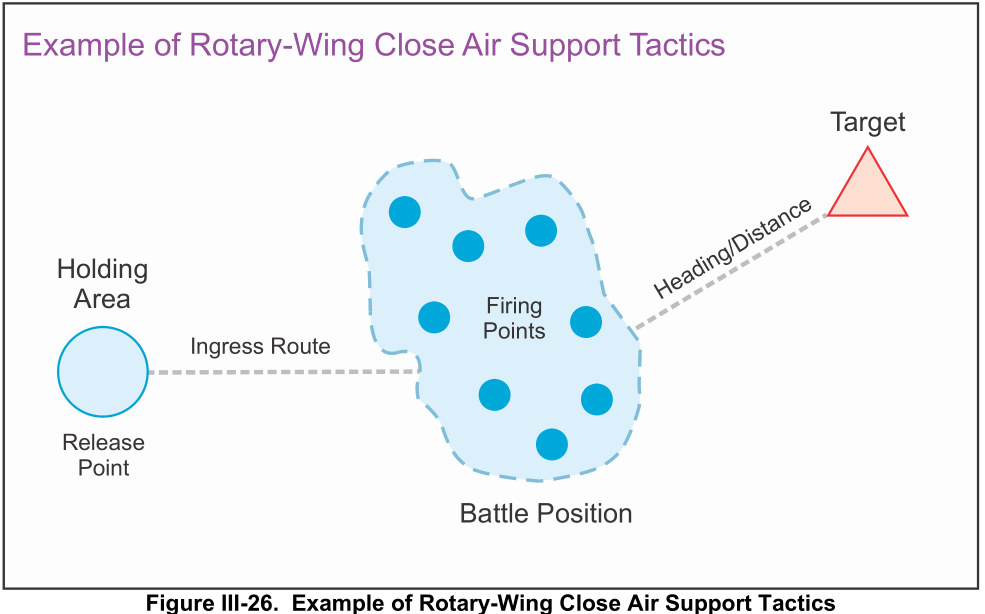
\includegraphics[width=\textwidth]{attackphase.png}
    \caption{Phase d'attaque.}
    \label{fig:attackphase}
\end{figure}

\subsection{Techniques de mouvement}

\e
    \item Du fait de la proximité de la menace, les \glspl{rw} utilisent le terrain pour se déplacer vers la \gls{bp}.
    \item Il existe 3 techniques de mouvement:
    \ee
        \item \titlepar{Travelling}{Le travelling est utilisé lorsque le contact avec l’ennemi est peu probable. La formation dans son ensemble progresse en suivant le terrain, avec des secteurs de scanning prédéfinis. Ce mode de déplacement permet une vitesse élevée dans des zones relativement sécurisées.}
        \item \titlepar{Travelling overwatch}{Le travelling overwatch est utilisé lorsque le contact avec l’ennemi est possible. La formation se déplace en vol de contour ou en vol NOE, avec un élément de tête en évolution constante et un élément de surveillance en retrait, qui se repositionne de manière à fournir un appui visuel et armé constant à l’élément de tête. Ce mode de déplacement lorsque la prudence est de mise mais la vitesse reste souhaitable.}
        \item \titlepar{Bounding Overwatch}{Le bounding overwatch est utilisé lorsque le contact avec l’ennemi est imminent. La formation se déplace en vol NOE, et est divisée en deux éléments, qui se déplacent alternativement, l’élément statique fournissant une couverture visuelle et armée constante à l’élément en mouvement à partir d’une position protégée.}
    \ed
\ed

\subsubsection{Résumé des types de mouvements}

\e
    \item Extrait du \jp:\\
    \begin{figure}[H]
        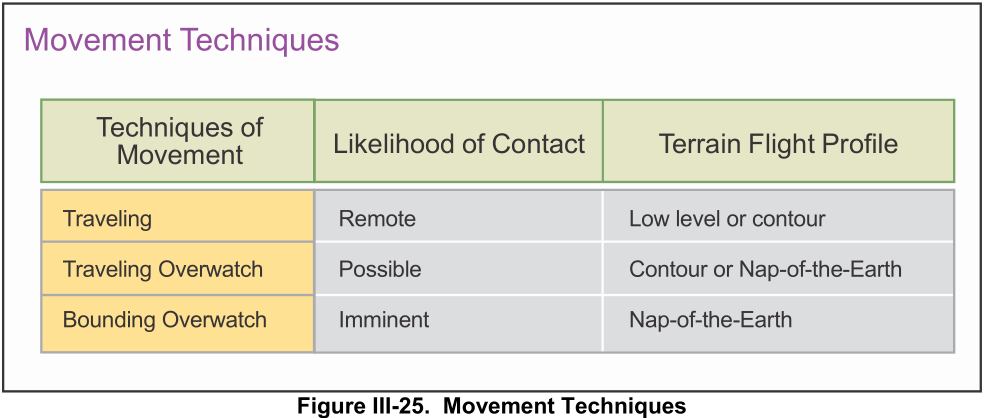
\includegraphics[width=\textwidth]{movementtypes.png}
        \caption{Types de mouvements pour les unités \gls{rw}.}
        \label{fig:movementtypes}
    \end{figure}
\ed

\subsubsection{Communications et contrôle}

\e
    \item
    Généralement, pendant la phase de pénétration, il sera préférable que la patrouille assure d’abord sa sécurité, ce qui peut entraîner une perte des communications de par la faible altitude nécessaire.
    \item La patrouille sera alors entièrement briefée avant de quitter la HA, et les communications reprendront une fois établi à la BP.
    \item Un relais aérien peut également être mis en place.
\ed

\section{Phase d’attaque}

\subsection{Contrôle}

\e
    \item Une fois la BP atteinte, le \gls{jtac}/\gls{faca} donnera les instructions finales à la patrouille.
    \item Les membres de la patrouilles choisissent leurs positions de tir, et restent masqués en attendant le \gls{tot}/\gls{ttt} ou l’ordre d’attaque
\ed

\subsection{Attaque}

\e
    \item Il existe 3 profils d’attaque: le tir stationnaire, le tir en route, et le tir plongeant.
\ed

\subsubsection{Tir stationnaire}

\e
    \item
    Le tir stationnaire s’effectue après un pop-up ou un stand-off, en vol stationnaire ou en vol vers l'avant très lent. \textbf{L’appareil doit rester stationnaire le moins longtemps possible}, et se repositionner une fois le tir effectué.
    \item
    Ce type de tir est le plus efficace pour délivrer les munitions guidées (Vikhrs). Le tir de munitions non guidée depuis le vol stationnaire c’est pas recommandé, car l’hélicoptère à une tendance à l’instabilité plus prononcée en vol stationnaire.
\ed

\subsubsection{Tir en route}

\e
    \item Le tir en route consiste à tirer les munitions en déplacement vers l’avant à altitude constante. Ce tir permet une plus grande stabilité de la plate-forme.
    \item
    Le tir en route permet de réduire la vulnérabilité de l’hélicoptère au tir d’armes de petit calibre, et améliore la capacité de réponse à un tir d’arme air-sol guidée contre l’hélicoptère de par l’énergie déjà acquise.
\ed

\subsubsection{Tir plongeant}

\e
    \item
    Le tir plongeant est effectué en déplacement vers l’avant et en descente, offre une précision accrue lors du tir de munitions non guidée, et permet à l’appareil de rester hors de l’enveloppe de tir des armes de petit calibre.

    \item
    La position élevée permet également une \gls{sa} très élevée, de par l’altitude plus importante. Cependant, cela implique une grande vulnérabilité aux missiles infrarouges.
\ed

\subsection{Désengagement et egress}

\e
    \item
    Une fois les actions nécessaires effectuées, ou lorsque le “play time” est écoulé, \textbf{le chef de patrouille devra effectuer un check-out avec le \gls{jtac}/\gls{faca}}, et quitter la zone via une route planifiée ou assignée.
    \item Les considération sur le retour sont identiques à celles de l’aller.
    \item Les \gls{rw}s peuvent utiliser un FARP pour le rearm/refuel, et ainsi allonger le temps pendant lequel ils sont à même de soutenir les troupes au sol alliées.
    \item \hfill
%    \customcolorbox[0.9\textwidth]{\colorboxred}{Important}{Lorsque la mission se termine, le chef de patrouille devra fournir un \acrlong{bda} et un MISREP au C2.}
%    \item \fcolorbox{red!20}{red!20}{I am a coloured box with a coloured frame}
%    \item \begin{tcolorbox}[box align=center, colframe=red!40!gray, boxrule=0pt, leftrule=5mm, colback=red!10!white] Lorsque la mission se termine, le chef de patrouille devra fournir un \gls{bda} et un \gls{misrep} au \gls{cc}.
%    \end{tcolorbox}
    \item \important{Lorsque la mission se termine, le chef de patrouille devra fournir un \gls{bda} et un \gls{misrep} au \gls{cc}.}

\ed





